% =============================================================================
% COPYRIGHT AND DISCLAIMER
% =============================================================================
% This file is provided as a convenience template for competition participants.
% By using it, you accept full responsibility for compliance with all applicable
% copyright, licensing, and usage rules of the Association for Computing
% Machinery (ACM) and of any LaTeX packages you load (including, without
% limitation, the "acmart" document class and related ACM materials).
%
% Consult ACM's official publication, template, and copyright policies before
% using this setup for any purpose other than this competition. Do not assume
% that this template may be reused, redistributed, or submitted elsewhere
% without independently verifying ACM's current rules.
%
% Use of the "acmart" class, the "sigconf" option, or ACM-style formatting in
% this template does NOT mean that this report, this competition, its organizers,
% or any resulting PDF is sponsored, endorsed, affiliated with, or published by
% ACM. ACM trademarks and branding remain the property of ACM.
%
% Template packages live in preamble.tex.
% Citations live in main.bib. Edit this file with your paper content.
% =============================================================================
%
% Numbers in this report are reproducible from the repository:
%   scripts/report_stats.py   -> reports/report_stats.json (stage PQ, bootstrap CIs, per-instrument PQ)
%   scripts/report_figures.py -> figures/pipeline.pdf, figures/examples.jpg
%   reports/geometry_audit.md, reports/experiment_decision.md (error analysis, G1/G2)

\documentclass[sigconf]{acmart}
% =============================================================================
% Template setup — participants normally do not edit this file.
% Author content belongs in main.tex; citations belong in main.bib.
% \documentclass lives in main.tex so Overleaf does not treat this file as root.
% =============================================================================

% --- Competition / non-ACM-submission friendly rights metadata -------------
\setcopyright{none}
\settopmatter{printacmref=false}
\acmConference[Kaggle Competition]{Filament Segmentation Challenge}{2026}{\href{https://www.kaggle.com/competitions/filament-segmentation-2026}{kaggle.com/competitions/filament-segmentation-2026}}
\acmBooktitle{Competition Report}
\acmDOI{}
\acmISBN{}

% --- Author guidance text --------------------------------------------------
% \guide{...} is gray italic while \guideStyletrue; omitted from the PDF if false.
% Flip the switch in main.tex after % =============================================================================
% Template setup — participants normally do not edit this file.
% Author content belongs in main.tex; citations belong in main.bib.
% \documentclass lives in main.tex so Overleaf does not treat this file as root.
% =============================================================================

% --- Competition / non-ACM-submission friendly rights metadata -------------
\setcopyright{none}
\settopmatter{printacmref=false}
\acmConference[Kaggle Competition]{Filament Segmentation Challenge}{2026}{\href{https://www.kaggle.com/competitions/filament-segmentation-2026}{kaggle.com/competitions/filament-segmentation-2026}}
\acmBooktitle{Competition Report}
\acmDOI{}
\acmISBN{}

% --- Author guidance text --------------------------------------------------
% \guide{...} is gray italic while \guideStyletrue; omitted from the PDF if false.
% Flip the switch in main.tex after % =============================================================================
% Template setup — participants normally do not edit this file.
% Author content belongs in main.tex; citations belong in main.bib.
% \documentclass lives in main.tex so Overleaf does not treat this file as root.
% =============================================================================

% --- Competition / non-ACM-submission friendly rights metadata -------------
\setcopyright{none}
\settopmatter{printacmref=false}
\acmConference[Kaggle Competition]{Filament Segmentation Challenge}{2026}{\href{https://www.kaggle.com/competitions/filament-segmentation-2026}{kaggle.com/competitions/filament-segmentation-2026}}
\acmBooktitle{Competition Report}
\acmDOI{}
\acmISBN{}

% --- Author guidance text --------------------------------------------------
% \guide{...} is gray italic while \guideStyletrue; omitted from the PDF if false.
% Flip the switch in main.tex after \input{preamble}.
%
% Do not use \guide{...} for \email{...}.
\usepackage{xcolor}
\newif\ifguideStyle
\guideStyletrue
\newcommand{\guide}[1]{%
  \ifguideStyle
    {\color{gray!65}\itshape #1}%
  \fi
}

% --- Math ------------------------------------------------------------------
% Do NOT load amssymb (or amsfonts): acmart already loads newtxmath, which
% defines the same symbols (e.g. \Bbbk) and causes a conflict on Overleaf.
% amsmath is already provided by acmart; mathtools extends it.
\usepackage{mathtools}

% --- Figures ---------------------------------------------------------------
% graphicx is already loaded by acmart
\usepackage{subcaption}

% --- Tables ----------------------------------------------------------------
% booktabs is already loaded by acmart
\usepackage{tabularx}
\usepackage{multirow}

% --- Bibliography style is set in main.tex (ACM-Reference-Format) ----------
.
%
% Do not use \guide{...} for \email{...}.
\usepackage{xcolor}
\newif\ifguideStyle
\guideStyletrue
\newcommand{\guide}[1]{%
  \ifguideStyle
    {\color{gray!65}\itshape #1}%
  \fi
}

% --- Math ------------------------------------------------------------------
% Do NOT load amssymb (or amsfonts): acmart already loads newtxmath, which
% defines the same symbols (e.g. \Bbbk) and causes a conflict on Overleaf.
% amsmath is already provided by acmart; mathtools extends it.
\usepackage{mathtools}

% --- Figures ---------------------------------------------------------------
% graphicx is already loaded by acmart
\usepackage{subcaption}

% --- Tables ----------------------------------------------------------------
% booktabs is already loaded by acmart
\usepackage{tabularx}
\usepackage{multirow}

% --- Bibliography style is set in main.tex (ACM-Reference-Format) ----------
.
%
% Do not use \guide{...} for \email{...}.
\usepackage{xcolor}
\newif\ifguideStyle
\guideStyletrue
\newcommand{\guide}[1]{%
  \ifguideStyle
    {\color{gray!65}\itshape #1}%
  \fi
}

% --- Math ------------------------------------------------------------------
% Do NOT load amssymb (or amsfonts): acmart already loads newtxmath, which
% defines the same symbols (e.g. \Bbbk) and causes a conflict on Overleaf.
% amsmath is already provided by acmart; mathtools extends it.
\usepackage{mathtools}

% --- Figures ---------------------------------------------------------------
% graphicx is already loaded by acmart
\usepackage{subcaption}

% --- Tables ----------------------------------------------------------------
% booktabs is already loaded by acmart
\usepackage{tabularx}
\usepackage{multirow}

% --- Bibliography style is set in main.tex (ACM-Reference-Format) ----------


% Guide styling: \guideStyletrue = show gray italic hints; \guideStylefalse = omit them
% \guideStyletrue
\guideStylefalse

\begin{document}

\title[Detect, then Refine]{Detect, then Refine: YOLO Instances with Full-Resolution Crop Refiners for Solar Filament Segmentation}  % Replace this with your title
\subtitle{A Solution to the Solar Filament Segmentation Challenge 2026} % DO NOT CHANGE


\author{Doğuş Can Korkmaz}
\affiliation{%
  \institution{Istanbul Technical University}  % <- Optional (remove if you are not currently affiliated with any institute)
  \city{Istanbul}
  \country{Türkiye}
}
\email{korkmazd18@itu.edu.tr}  % <- Replace with your own email

\author{Tuğçe Keskin}
\affiliation{%
  \institution{Istanbul Technical University}  % <- Optional (remove if you are not currently affiliated with any institute)
  \city{Istanbul}
  \country{Türkiye}
}
\email{keskint26@itu.edu.tr}   % <- Replace with your own email

\begin{abstract}
    This report describes our solution to the Solar Filament Segmentation Challenge~2026, a Kaggle competition on automatic segmentation of solar filaments in GONG H-$\alpha$ observations. A YOLO11m-seg detector at 1536\,px with flip test-time augmentation proposes filament instances; a U-Net and a LoRA-tuned Segment Anything model then re-predict every mask from a full-resolution crop, and their probabilities are averaged. The system reaches a panoptic quality (PQ) of 0.474 (95\% CI 0.457--0.492) on a date-grouped validation fold and 0.40 on the public leaderboard. We quantify the contribution of each stage with paired bootstrap tests, analyse the remaining errors (most near misses are correctly located but too short) and report two geometry corrections that did not help.
\end{abstract}

\maketitle

\ifguideStyle
\noindent{\color{gray!65}\itshape
Guide mode is on.}
\par\medskip
\fi

\guide{Please limit your report to four (4) pages, excluding the Acknowledgment and References sections. Throughout this document, please follow these considerations:
\begin{itemize}
    \item Do not alter any text that is currently in black color (except for the emails under authors' name).
    \item Replace all gray text with your own.
    \item When you are done with the report, please replace \texttt{\textbackslash guideStyletrue} with \texttt{\textbackslash guideStylefalse}, to remove any gray text. Alternatively, you can remove any text wrapped in \texttt{\textbackslash guide\{\}},
    \item Be as succinct as possible, and only provide details regarding your own work. For example, there is no need to discuss what solar filaments are, or why filament segmentation matters.
    \item If you must, you can add extra sections.
\end{itemize}}


% ==================================== %
%              INTRODUCTION            %
% ==================================== %
\section{Introduction}
    This report goes over the details of our submitted solution to the Solar Filament Segmentation Challenge~2026 \cite{filament-segmentation-2026}. The challenge, launched on July~10,~2026, is organized by the Earth-Space AI Research (ESAIR) Lab\footnote{\href{https://www.esairlab.com/home}{www.esairlab.com/}}. This challenge utilizes the MAGFiLO dataset for evaluation of the segmentation algorithms \cite{ahmadzadeh2024dataset}. The task is instance segmentation of every filament in a 2048$\times$2048 full-disk image. A prediction is scored separately against each annotator's labelling of an image: it is a true positive (TP) if its IoU with an annotated filament exceeds 0.5, and the panoptic quality \cite{kirillov2019panoptic} is pooled over all annotator views as $\mathrm{PQ}=\sum \mathrm{IoU}_{TP}/(TP+\tfrac12 FP+\tfrac12 FN)$.

    Our design follows from two observations. First, filaments are thin and long, so the 1/4-resolution masks of a single-stage detector are too coarse; we therefore separate \emph{finding} instances (a YOLO detector) from \emph{drawing} them (crop refiners at full resolution). Second, annotators disagree substantially, which bounds what any model can score and makes small validation differences unreliable; we therefore report confidence intervals and adopt a change only when it is clearly outside the noise. The full pipeline is shown in Fig.~\ref{fig:pipeline}. Code, weights and a one-command inference script are available at \url{https://github.com/tugcekeskin/solar-filament-segmentation-2026-vprg}.


% ==================================== %
%              METHODOLOGY             %
% ==================================== %
\begin{figure*}[t]
  \centering
  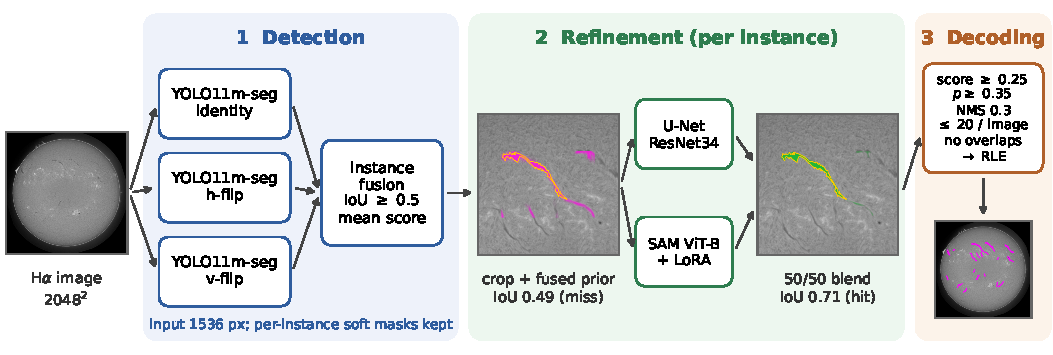
\includegraphics[width=\textwidth]{figures/pipeline.pdf}
  \caption{End-to-end inference pipeline, illustrated on a validation image. Each image is passed through the detector three times (identity, horizontal and vertical flip) and the instances are fused. For every instance, a full-resolution crop and the fused soft mask (magenta) are re-drawn by two refiners whose probabilities are averaged (green); the yellow outline is the closest annotation. In this example, chosen to show the effect, refinement removes spurious branches and raises the IoU from 0.49 (a miss) to 0.71 (a hit). Decoding produces non-overlapping run-length-encoded masks.}
  \label{fig:pipeline}
\end{figure*}

\section{Methodology}\label{sec:methodology}

\subsection{Data and sampling}
The training set has 707 images with 1154 annotator views (411 images labelled once, 145 twice, 151 three times) and 8199 filament polygons in four chirality categories. Because the metric is class-agnostic, all categories are merged into one class. Each annotator view is a separate training sample with its own labels, so multiply-annotated images contribute every view; we found no gain from consensus labels. We split the images into five folds grouped by observation date, so that the views of one image and images of the same day never straddle the split, and use fold~0 for validation (142 images, 220 views, 1545 filaments; 565 training images, 934 views). All design choices and post-processing thresholds were selected on this fold; the test set was used only for inference. No external data were used. Pre-processing is minimal: the grey-level JPEG is replicated to three channels and resized by the detector; flat-fielding and CLAHE channels did not help (Table~\ref{tab:abl}).

\subsection{Detector}
We use YOLO11m-seg \cite{yolo11}, which predicts boxes and YOLACT-style prototype masks \cite{bolya2019yolact} at 1/4 of the input resolution, initialised from COCO \cite{lin2014coco} weights. It is trained as a single class at 1536\,px for 80 epochs with AdamW \cite{loshchilov2019adamw} (lr 10$^{-3}$, cosine decay to 10$^{-5}$, weight decay $5\cdot10^{-4}$, 3 warm-up epochs, batch 2, mixed precision, seed 0). Augmentation: horizontal and vertical flips ($p=0.5$), rotation $\pm15^\circ$, scale $\pm0.3$, translation 0.05, brightness $\pm0.3$, mosaic 0.5 switched off for the last 15 epochs. Input resolution mattered more than model size: from 1024 to 1536\,px PQ rose by about 0.01, while YOLO11s$\rightarrow$YOLO11m added 0.002--0.009 and 1792\,px nothing.

\subsection{Test-time augmentation and fusion}
Every image is predicted as is, flipped horizontally and flipped vertically, keeping the soft (probability) mask of every instance with score $\ge 0.01$. The three passes are matched greedily by mask IoU $\ge 0.5$; matched instances average their soft masks, and the fused score is the mean over the three passes, with a missing pass counting as zero. Instances that only one pass finds are thus down-weighted.

\subsection{Crop refiners}
For every fused instance we cut a square window around its mask bounding box, padded by 25\% of the longer side, from the full-resolution image and resize it to 256$\times$256. A refiner receives two channels, the per-crop standardised image and the fused soft mask as a prior, and predicts the instance mask in the same frame, which is pasted back. Two refiners are used:
\begin{itemize}
  \item \textbf{U-Net} \cite{ronneberger2015unet} with an ImageNet-pretrained ResNet34 encoder \cite{he2016resnet, iakubovskii2019smp}; 25 epochs, batch 32, AdamW (lr $3\cdot10^{-4}$, cosine), loss BCE + soft Dice.
  \item \textbf{SAM ViT-B} \cite{kirillov2023sam} with LoRA \cite{hu2022lora} (rank 16, $\alpha=32$) on every attention projection of the frozen image encoder, and the full prompt encoder and mask decoder trainable (4.65\,M parameters). The crop is contrast-stretched and upsampled to 1024\,px; the prior is given as a box prompt and as the mask prompt, whose 256$^2$ frame maps 1:1 to the output. 3 epochs, batch 2, lr 10$^{-4}$, same loss.
\end{itemize}
Both are trained on the training fold only. Training pairs are the detector's own proposals on training images matched to each view's filaments (IoU $\ge 0.2$, target = that view's mask), plus 30\% synthetic priors made from ground-truth masks by random dilation (1--4\,px), shifts ($\pm$3\,px), Gaussian blur ($\sigma$ 1--4) and edge sharpness. At inference each refiner averages its prediction with that of the horizontally flipped crop, and the two refiners' probabilities are averaged with equal weight. On held-out training crops the U-Net raises the mask IoU of the prior from 0.551 to 0.657.

\subsection{Decoding}
Instances with fused score $\ge 0.25$ are binarised at probability 0.35; masks smaller than 100\,px are dropped, mask-NMS at IoU 0.3 is applied and at most 20 instances per image are kept. Remaining overlaps are resolved pixel-wise in favour of the higher-scoring instance, so the submission never contains overlapping masks. All thresholds were chosen by grid search on the validation fold.

Because views are scored separately and without one-to-one matching, emitting a candidate $c$ increases PQ exactly when its expected matched IoU, $\frac1V\sum_v \mathrm{IoU}_v(c)\,[\mathrm{IoU}_v(c)>0.5]$, exceeds PQ/2. Selection is therefore a calibrated threshold on a good estimate of this quantity; the detector score already is one, and a learned second-stage rescorer did not improve on it (Table~\ref{tab:abl}).

\begin{figure*}[t]
  \centering
  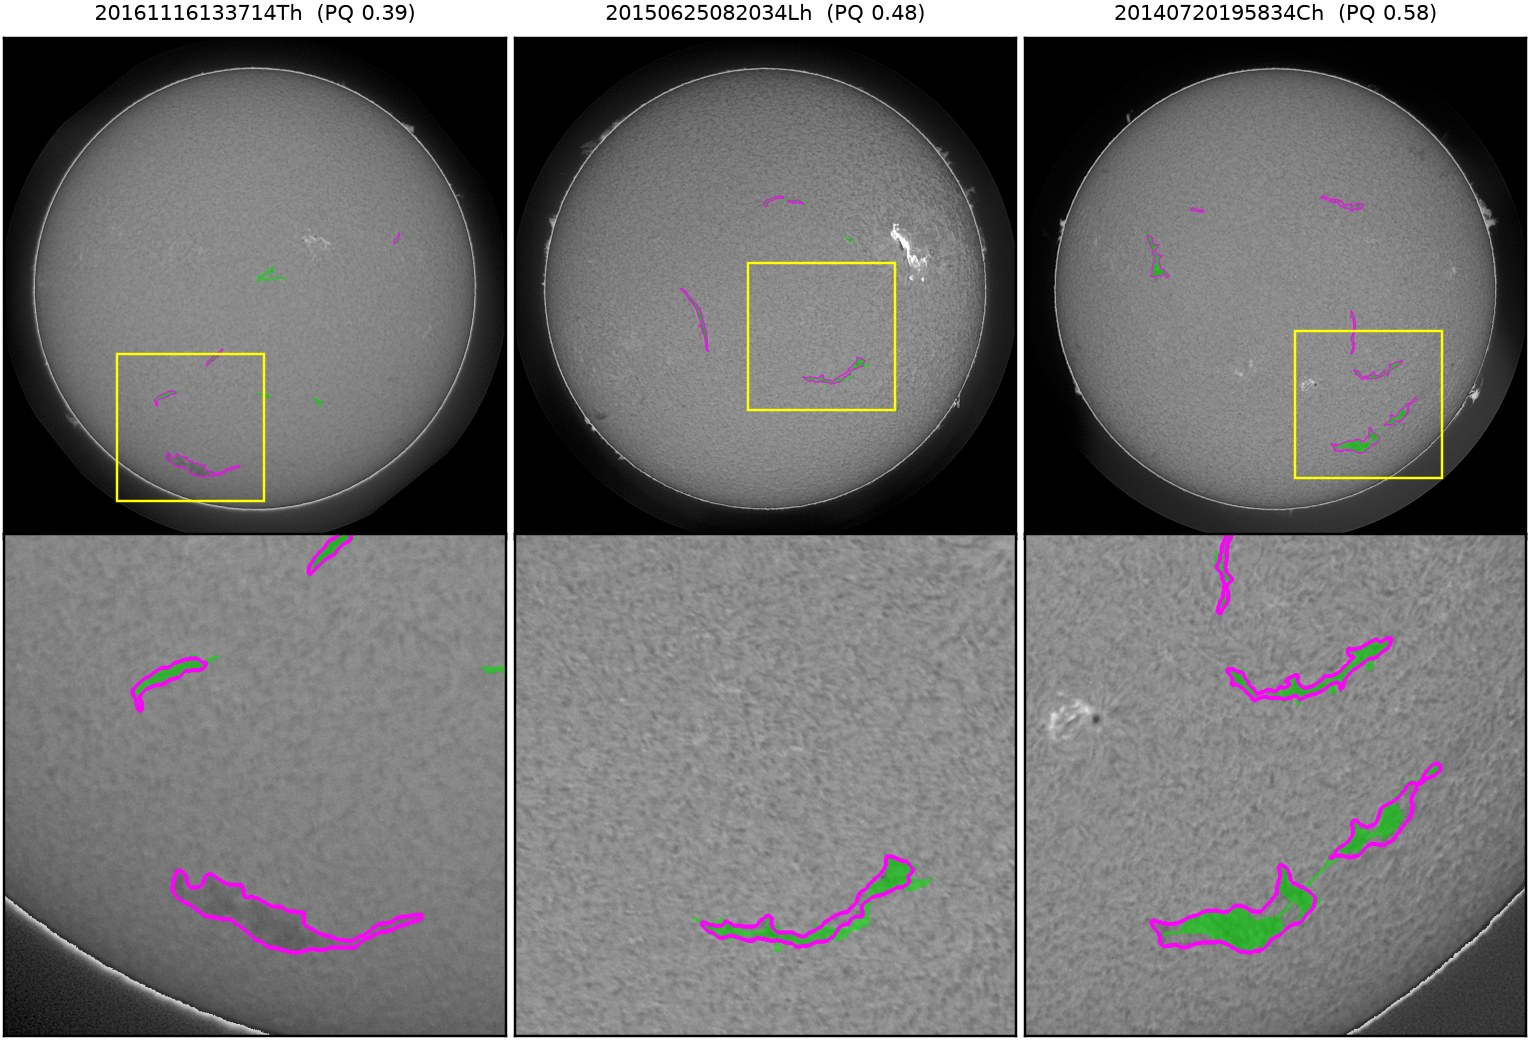
\includegraphics[width=0.94\textwidth]{figures/examples.jpg}
  \caption{Final predictions (magenta outlines) and one annotator's labels (green fill) on three validation images at the 20th, 50th and 80th percentile of per-image PQ; bottom row: zoom on the yellow box. Left: a clearly visible filament that this annotator did not mark counts as a false positive. Middle and right: boundaries largely agree; the remaining differences are where a filament ends and whether neighbouring segments form one filament.}
  \label{fig:examples}
\end{figure*}


% ==================================== %
%              EVALUATION              %
% ==================================== %
\section{Evaluation}\label{sec:evaluation}

\subsection{Strategy}
We re-implemented the organisers' evaluation (per-view scoring, strict IoU $>0.5$, pooled PQ) and unit-tested it against their self-evaluation notebook. Uncertainty is estimated with a bootstrap over validation images (2000 resamples; all views of an image are resampled together), and stage gains with a paired bootstrap on the same resamples. Training noise is estimated by re-running the full pipeline with a second detector seed.

\begin{table}[t]\centering\small
\caption{Validation PQ (fold 0, 142 images) with 95\% bootstrap CIs, and the paired gain of the final pipeline over each intermediate stage. Each stage uses its own calibrated thresholds.}\label{tab:main}
\setlength{\tabcolsep}{3pt}
\resizebox{\columnwidth}{!}{%
\begin{tabular}{lccc}\toprule
Pipeline & PQ {\scriptsize[95\% CI]} & TP/FP/FN & final $-$ stage \\\midrule
YOLO11m, one pass & 0.452 {\scriptsize[.434, .469]} & 939/343/606 & +0.022 {\scriptsize[.016, .029]} \\
+ flip TTA & 0.462 {\scriptsize[.446, .479]} & 988/393/557 & +0.012 {\scriptsize[.007, .017]} \\
+ U-Net refiner & 0.468 {\scriptsize[.450, .484]} & 994/393/551 & +0.007 {\scriptsize[.003, .011]} \\
+ SAM-LoRA blend & \textbf{0.474} {\scriptsize[.457, .492]} & 1003/379/542 & -- \\\bottomrule
\end{tabular}}\end{table}

\subsection{Results}
Table~\ref{tab:main} shows that every stage adds a gain whose paired 95\% interval excludes zero; together they add 0.022 PQ over the single-pass detector. The absolute PQ is uncertain to about $\pm$0.017 because of image-to-image variance, and retraining the detector with another seed moves the full pipeline by about 0.01 (0.464 vs 0.474), so differences below $\approx$0.005 between configurations were treated as noise. On the public leaderboard the final pipeline scores 0.40 and the detector with flip TTA 0.39. The validation--leaderboard gap is similar for all our models and for public baselines, which suggests a difference in labelling density on the test set rather than overfitting. Per instrument (Bh, Ch, Lh, Mh, Th, Uh) PQ ranges from 0.438 [0.398, 0.479] (Mh) to 0.497 [0.452, 0.546] (Th), with overlapping intervals.

\paragraph{Human agreement.} Scoring one annotator's view as a prediction against the other views of the same image gives PQ 0.337. On multiply-annotated images, our predictions score 0.479 against a held-out view, whereas selecting our candidates with the \emph{other} annotators' labels scores only 0.452--0.471. Our confidence thus predicts an unseen annotator better than the other annotators do, and much of the remaining error is annotator-specific (Fig.~\ref{fig:examples}, left).

\begin{table}[t]\centering\small
\caption{Changes that did not help (validation PQ unless marked; reference pipeline of the time in parentheses). Validation gains inside seed noise did not carry over to the public leaderboard.}\label{tab:abl}
\setlength{\tabcolsep}{4pt}
\begin{tabular}{lc}\toprule
Change & PQ \\\midrule
imgsz 1792 & 0.462 (0.468) \\
flat-field + CLAHE input channels & 0.460 (0.468) \\
multi-model or multi-seed detector ensembles & 0.462--0.466 (0.468) \\
multi-scale TTA (1280/1536/1792) & 0.472 (0.474) \\
copy-paste, loss weights, consensus labels & within $\pm$0.006 \\
two-class detector (identified / unidentified) & 0.462--0.468 (0.474) \\
positive-unlabelled loss (ignore unlabelled candidates) & 0.466 (0.474) \\
per-instrument thresholds (5-fold CV) & 0.468 (0.474) \\
learned second-stage rescorer (gradient boosting) & 0.469 (0.474) \\
path completion from fragment endpoints & 0.380--0.474 (0.474) \\
Skeleton Recall loss \cite{kirchhoff2024skeleton} in the U-Net & 0.474--0.477 (0.474) \\
U-Net on prior-only crop windows & 0.475--0.477 (0.474) \\
\quad same, public leaderboard & 0.39 (0.40) \\
detector retrained on all 707 images, public LB & 0.39 (0.39) \\
Mask R-CNN + U-Net refiner (public baseline) & 0.416 (0.474) \\\bottomrule
\end{tabular}\end{table}

\subsection{Error analysis}
At the decoding used in the error audit (score $\ge 0.2$; PQ 0.474, TP 1060, FP 485, FN 485), half of the missed filaments (240) have no overlapping prediction at all; 80 overlap with IoU below 0.3, and 165 are near misses with IoU 0.3--0.5. Among the near misses, 39\% are \emph{fragments} (the prediction is precise but covers less than 60\% of the filament), 19\% are shifted, 16\% too large, 15\% merge two labelled filaments and 12\% split one. Fragments are short rather than thin: their skeleton is a median 0.54 of the label's length (113\,px missing) while their width ratio is 0.90, and every fragmented label is a single polygon. Oracle repairs that use the labels bound the potential of geometry: growing each fragment inside its label by up to 96\,px gives +0.024 PQ, perfect geometry on all near misses +0.069.

We tested two corrections aimed at fragments. (i) \emph{Path completion}: a shortest path from each skeleton endpoint along dark, direction-consistent pixels, forbidden to cross other instances, the limb or sunspots, trimmed where darkness falls below $\alpha$ times the instance's own and painted at its width. All settings lowered PQ ($-0.003$ to $-0.029$; a greedy tracer down to $-0.094$): darkness beyond an endpoint does not predict where an annotator ended a filament. (ii) A \emph{Skeleton Recall} loss in the U-Net gained at most +0.003, inside the 0.005 spread between two plain retrains of the refiner.

\subsection{Strengths, weaknesses and possible improvements}
\textbf{Strengths:} every component is standard and pretrained, training takes about 4\,h on one 16\,GB GPU (detector 1.3\,h, U-Net 0.2\,h, SAM 2.5\,h), inference on the 180 test images takes a few minutes, and every stage's contribution is statistically supported. Separating detection from full-resolution mask drawing makes the masks thin enough for the IoU $>0.5$ criterion. \textbf{Weaknesses:} a third of the misses are never proposed; the refiners only see a window around the proposal, so they cannot extend a fragment beyond it; and the model has no notion of which faint structures an annotator would skip. \textbf{Possible improvements:} refiners with larger, orientation-aligned windows; training against all views of an image jointly, so that the model learns the distribution of annotator choices instead of averaging them; and a detector that sees the full 2048\,px image.


% ==================================== %
%            ACKNOWLEDGMENT            %
% ==================================== %
\section{Acknowledgment}\label{sec:acknowledgment}
    % Do not change
    The organization of the Filament Segmentation Challenge 2026 is partially supported by the U.S. National Science Foundation (NSF) under Grant No. 2209912 and 2433781, directorate for Computer and Information Science and Engineering (CSE), and Office of Advanced Cyberinfrastructure (OAC), and Grant No. 2511630, AST Division Of Astronomical Sciences and MPS Directorate for Mathematical and Physical Sciences.

    The Filament Segmentation Challenge 2026 is sponsored by the U.S. National Science Foundation (NSF) National Solar Observatory (NSO).

    This work utilizes GONG data obtained by the NSO Integrated Synoptic Program, managed by the National Solar Observatory, which is operated by the Association of Universities for Research in Astronomy (AURA), Inc. under a cooperative agreement with the National Science Foundation and with contribution from the National Oceanic and Atmospheric Administration. The GONG network of instruments is hosted by the Big Bear Solar Observatory, High Altitude Observatory, Learmonth Solar Observatory, Udaipur Solar Observatory, Instituto de Astrofísica de Canarias, and Cerro Tololo Interamerican Observatory.

\bibliographystyle{ACM-Reference-Format}
\bibliography{main}

\end{document}
